% !TeX program = xelatex
\documentclass[12pt,a4paper]{article}
\usepackage{fontspec}
\setmainfont{Times New Roman}[Path=C:/Windows/Fonts/,UprightFont=times.ttf,BoldFont=timesbd.ttf,ItalicFont=timesi.ttf,BoldItalicFont=timesbi.ttf]
\usepackage{amsmath,amssymb,amsfonts}
\usepackage[left=1.5cm,right=1.5cm,top=1.4cm,bottom=1.6cm,headheight=17pt]{geometry}
\usepackage{enumitem,array,graphicx,tikz,fancyhdr,needspace}
\usetikzlibrary{arrows.meta,calc,patterns}
% Sửa số đề và số trang đề thực tế sau khi biên dịch/tách PDF.
\newcommand{\soDe}{12}
\newcommand{\soTrangDe}{4}
\newcommand{\maDe}{\ifnum\soDe<1000 0\fi\ifnum\soDe<100 0\fi\ifnum\soDe<10 0\fi\soDe}
\pagestyle{fancy}
\fancyhf{}
\lhead{\small\textbf{ÔN TẬP GIỮA KÌ I}}
\rhead{\small\textit{Biên soạn: Dương Gia Bảo}}
\rfoot{\small Trang \thepage/\soTrangDe\ - Mã đề: \maDe}
\renewcommand{\headrulewidth}{0.4pt}
\fancypagestyle{answers}{\rfoot{\small Trang \thepage\ - Mã đề: \maDe}}
\fancypagestyle{firstpage}{\fancyhead{}\renewcommand{\headrulewidth}{0pt}}
\setlength{\parindent}{0pt}
\setlength{\parskip}{2.5pt}
\setlength{\emergencystretch}{1em}
\setlist[enumerate,1]{label=\textbf{Câu \arabic*:},leftmargin=*,itemsep=5pt,topsep=2pt}
\setlist[enumerate,2]{label=\alph*),leftmargin=*,itemsep=2pt,topsep=2pt}
\newcommand{\bonpa}[4]{\par\nobreak\smallskip\nobreak\noindent
\begin{tabular}{@{}p{0.47\linewidth}p{0.47\linewidth}@{}}
\textbf{A.} #1 & \textbf{B.} #2\\[8pt]
\textbf{C.} #3 & \textbf{D.} #4\end{tabular}}
\newcommand{\loigiai}[1]{\par\medskip\Needspace{4\baselineskip}\noindent\textbf{#1}\par\nobreak}
\newcommand{\otraloi}{\par\nobreak\smallskip\noindent\textit{Trả lời:}\quad\fbox{\rule{0pt}{11pt}\makebox[0.3cm]{}}\,\fbox{\rule{0pt}{11pt}\makebox[0.3cm]{}}\,\fbox{\rule{0pt}{11pt}\makebox[0.3cm]{}}\,\fbox{\rule{0pt}{11pt}\makebox[0.3cm]{}}}
\begin{document}
\thispagestyle{firstpage}
\noindent
\begin{minipage}[t]{0.35\textwidth}
    \centering
    {\fontsize{13}{15}\selectfont\textbf{ÔN TẬP GIỮA KÌ I}}\\[4pt]
    \textit{Biên soạn: Dương Gia Bảo}\\[5pt]
    \setlength{\fboxrule}{0.8pt}%
    \setlength{\fboxsep}{4pt}%
    \fbox{\begin{minipage}{0.83\linewidth}
        \centering
        {\fontsize{13}{15}\selectfont\textbf{ĐỀ ÔN TẬP}\\[2pt]\textbf{CHƯƠNG I VÀ II}}\\[4pt]
        \textit{(Đề thi gồm có \ifnum\soTrangDe<10 0\fi\soTrangDe\ trang)}
    \end{minipage}}
\end{minipage}\hfill
\begin{minipage}[t]{0.63\textwidth}
    \centering
    {\fontsize{13}{15}\selectfont\textbf{ÔN TẬP KIỂM TRA GIỮA KÌ I}\\[2pt]
    \textbf{NĂM HỌC 2026 - 2027}}\\[5pt]
    {\fontsize{14}{16}\selectfont\textbf{Môn: TOÁN - Lớp 12 (ĐỀ SỐ \soDe)}}\\[4pt]
    {\fontsize{11.5}{13}\selectfont\textit{Thời gian làm bài: 90 phút, không kể thời gian giao đề}}\\[5pt]
    \setlength{\fboxrule}{0.8pt}%
    \setlength{\fboxsep}{5pt}%
    \fbox{\makebox[3cm]{\fontsize{14}{16}\selectfont\textbf{Mã đề: \maDe}}}
\end{minipage}
\par\vspace{2pt}
\hrule height 0.6pt
\vspace{3pt}
\noindent\textit{Họ và tên học sinh:}\dotfill\hspace{1cm}\textit{Lớp:}\makebox[3.5cm]{\dotfill}
\par\vspace{2pt}
\hrule height 0.6pt
\vspace{3pt}

\section*{\large PHẦN I. Câu trắc nghiệm nhiều phương án lựa chọn}
\textit{Thí sinh trả lời từ câu 1 đến câu 12. Mỗi câu chỉ chọn một phương án.}
\begin{enumerate}
\item Cho hàm số $y=x^3-3x^2-9x+2$. Hàm số đã cho nghịch biến trên khoảng nào dưới đây?
\bonpa{$(-1;3)$.}{$(3;+\infty)$.}{$(-\infty;-1)$.}{$(-2;4)$.}

\item Cho hàm số $y=-x^3+3x^2+1$. Giá trị cực đại của hàm số đã cho bằng
\bonpa{$1$.}{$5$.}{$2$.}{$0$.}

\item Giá trị lớn nhất của hàm số $f(x)=\dfrac{x-2}{x+1}$ trên đoạn $[0;3]$ bằng
\bonpa{$-2$.}{$0$.}{$\dfrac{1}{4}$.}{$1$.}

\item Đường tiệm cận xiên của đồ thị hàm số $y=\dfrac{x^2-3x+1}{x-2}$ có phương trình là
\bonpa{$y=x+1$.}{$y=x-2$.}{$y=2x-1$.}{$y=x-1$.}

\item Tọa độ giao điểm $I$ của hai đường tiệm cận của đồ thị hàm số $y=\dfrac{3x-1}{x+2}$ là
\bonpa{$I(2;3)$.}{$I(-2;3)$.}{$I(-2;-1)$.}{$I(3;-2)$.}

\item Đường cong trong hình vẽ bên là đồ thị của hàm số nào dưới đây?
\par\nobreak\smallskip
\begin{minipage}[c]{0.62\linewidth}
\bonpa{$y=\dfrac{x^2+2x+2}{x+1}$.}{$y=\dfrac{x^2-2x+2}{x-1}$.}{$y=\dfrac{x^2+x+2}{x+1}$.}{$y=\dfrac{x^2+2x-1}{x+1}$.}
\end{minipage}\hfill
\begin{minipage}[c]{0.36\linewidth}\centering
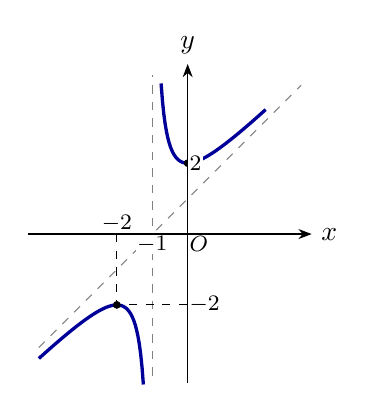
\begin{tikzpicture}[x=0.45cm,y=0.45cm,>=Stealth]
\draw[->] (-4.5,0)--(3.5,0) node[right] {$x$};
\draw[->] (0,-4.2)--(0,4.8) node[above] {$y$};
\draw[dashed,gray] (-1,-4.0)--(-1,4.5);
\draw[dashed,gray] (-4.2,-3.2)--(3.2,4.2);
\draw[very thick,blue!60!black,domain=-4.2:-1.25,samples=80] plot (\x,{(\x*\x+2*\x+2)/(\x+1)});
\draw[very thick,blue!60!black,domain=-0.75:2.2,samples=80] plot (\x,{(\x*\x+2*\x+2)/(\x+1)});
\draw[dashed] (-2,0)--(-2,-2)--(0,-2);
\fill (0,2) circle (1.4pt);
\fill (-2,-2) circle (1.4pt);
\node[below right,fill=white,inner sep=0.5pt] at (0,0) {\footnotesize $O$};
\node[below,fill=white,inner sep=0.5pt] at (-1,0) {\footnotesize $-1$};
\node[above,fill=white,inner sep=0.5pt] at (-2,0) {\footnotesize $-2$};
\node[right,fill=white,inner sep=0.5pt] at (0,-2) {\footnotesize $-2$};
\node[right,fill=white,inner sep=0.5pt] at (0,2) {\footnotesize $2$};
\end{tikzpicture}
\end{minipage}
\end{enumerate}

\newpage
\begin{enumerate}[start=7]
\item Số lượng sản phẩm bán ra của một doanh nghiệp phụ thuộc vào giá bán $p$ (nghìn đồng) theo hàm cầu $D(p)=800-10p$ với $20\le p\le 70$. Doanh thu từ việc bán sản phẩm là $R(p)=p\cdot D(p)=800p-10p^2$. Để doanh thu đạt giá trị lớn nhất thì giá bán $p$ bằng bao nhiêu nghìn đồng?
\bonpa{$35$.}{$50$.}{$40$.}{$45$.}

\item Cho tứ diện $ABCD$. Gọi $M$ là trung điểm của đoạn thẳng $CD$. Tổng hai vectơ $\vec{AC}+\vec{AD}$ bằng vectơ nào dưới đây?
\bonpa{$\vec{AM}$.}{$\vec{CD}$.}{$2\vec{MC}$.}{$2\vec{AM}$.}

\item Trong không gian $Oxyz$, cho điểm $A(2;-3;5)$. Hình chiếu vuông góc của điểm $A$ lên mặt phẳng tọa độ $(Oxy)$ có tọa độ là
\bonpa{$(2;-3;0)$.}{$(0;0;5)$.}{$(2;0;5)$.}{$(0;-3;5)$.}

\item Trong không gian $Oxyz$, cho hai vectơ $\vec{a}=(1;-2;3)$ và $\vec{b}=(2;1;-1)$. Tọa độ của vectơ $\vec{u}=2\vec{a}+\vec{b}$ là
\bonpa{$(3;-1;2)$.}{$(4;-3;5)$.}{$(0;-5;7)$.}{$(4;-1;5)$.}

\item Trong không gian $Oxyz$, cho hai vectơ $\vec{u}=(1;0;1)$ và $\vec{v}=(0;1;-1)$. Côsin của góc giữa hai vectơ $\vec{u}$ và $\vec{v}$ bằng
\bonpa{$\dfrac{1}{2}$.}{$\dfrac{\sqrt{2}}{2}$.}{$-\dfrac{\sqrt{2}}{2}$.}{$-\dfrac{1}{2}$.}

\item Trong không gian $Oxyz$, cho hai điểm $A(1;3;-2)$ và $B(3;2;0)$. Độ dài đoạn thẳng $AB$ bằng
\bonpa{$\sqrt{5}$.}{$9$.}{$3$.}{$\sqrt{21}$.}
\end{enumerate}

\vspace{3pt}
\section*{\large PHẦN II. Câu trắc nghiệm đúng hoặc sai}
\textit{Thí sinh trả lời từ câu 1 đến câu 4. Trong mỗi ý a), b), c), d) ở mỗi câu, thí sinh chọn đúng hoặc sai.}
\begin{enumerate}
\item Cho hàm số $y=f(x)=\dfrac{x^2-3x+6}{x-1}$.
\begin{enumerate}
\item Tập xác định của hàm số là $D=\mathbb{R}\setminus\{1\}$.
\item Đạo hàm của hàm số là $f'(x)=\dfrac{x^2-2x-3}{(x-1)^2}$.
\item Đồ thị hàm số có đường tiệm cận xiên là đường thẳng $y=x+2$.
\item Khoảng cách giữa hai điểm cực trị của đồ thị hàm số bằng $4\sqrt{5}$.
\end{enumerate}
\end{enumerate}

\newpage
\begin{enumerate}[start=2]
\item Một xưởng sản xuất thiết bị gia dụng sản xuất $x$ trăm sản phẩm mỗi tuần ($0 < x \le 20$). Tổng chi phí sản xuất (tính bằng triệu đồng) được cho bởi hàm số $C(x)=x^3-15x^2+180x+80$. Doanh thu từ việc bán sản phẩm (tính bằng triệu đồng) được cho bởi hàm số $R(x)=300x-6x^2$. Lợi nhuận hàng tuần của xưởng là $P(x)=R(x)-C(x)$.
\begin{enumerate}
\item Chi phí cố định ban đầu của xưởng (khi chưa sản xuất sản phẩm nào) là $80$ triệu đồng.
\item Doanh thu của xưởng khi bán được $5$ trăm sản phẩm là $1350$ triệu đồng.
\item Hàm lợi nhuận hàng tuần của xưởng theo số lượng $x$ là $P(x)=-x^3+9x^2+120x-80$.
\item Xưởng đạt lợi nhuận lớn nhất trong tuần khi sản xuất $12$ trăm sản phẩm.
\end{enumerate}

\item Trong không gian $Oxyz$, cho ba điểm $A(1;2;0)$, $B(2;0;2)$ và $C(-1;3;1)$.
\begin{enumerate}
\item Tọa độ của vectơ $\vec{AB}$ là $\vec{AB}=(1;-2;2)$.
\item Độ dài cạnh $AB$ bằng $3$.
\item Trọng tâm $G$ của tam giác $ABC$ có tọa độ là $G\left(\dfrac{2}{3};\dfrac{5}{3};1\right)$.
\item Tọa độ điểm $D$ để tứ giác $ABCD$ là hình bình hành là $D(-2;5;1)$.
\end{enumerate}

\item Một quả cầu trang trí nghệ thuật có trọng lượng $P=120\text{ N}$ được giữ thăng bằng trong không gian bằng ba sợi dây cáp mảnh, nhẹ, không dãn $OA, OB, OC$. Ba đầu dây được cố định tại ba điểm $A, B, C$ trên trần nhà nằm ngang tạo thành một tam giác đều, còn ba đầu kia cùng buộc vào móc treo quả cầu tại điểm $O$. Chọn hệ trục toạ độ $Oxyz$ có gốc tại $O$, tia $Oz$ hướng thẳng đứng lên trần nhà (ngược hướng với trọng lực). Khi đó trọng lực tác dụng lên quả cầu là $\vec{P}=(0;0;-120)$ (đơn vị: N). Lực căng tác dụng lên móc treo $O$ bởi ba sợi dây lần lượt là $\vec{F}_1, \vec{F}_2, \vec{F}_3$. Biết rằng ba lực này có cùng độ lớn $|\vec{F}_1|=|\vec{F}_2|=|\vec{F}_3|=F$, cùng tạo với phương thẳng đứng (trục $Oz$) một góc $45^\circ$, và hình chiếu của ba lực lên mặt phẳng nằm ngang $Oxy$ đôi một hợp với nhau góc $120^\circ$.
\begin{enumerate}
\item Vì quả cầu ở trạng thái cân bằng nên ta có hệ thức $\vec{F}_1+\vec{F}_2+\vec{F}_3+\vec{P}=\vec{0}$.
\item Hợp lực của ba lực căng dây $\vec{F}=\vec{F}_1+\vec{F}_2+\vec{F}_3$ có phương thẳng đứng hướng lên và có độ lớn bằng $120\text{ N}$.
\item Độ lớn của mỗi lực căng dây là $F=40\sqrt{2}\text{ N}$.
\item Góc tạo bởi mỗi sợi dây cáp và mặt phẳng nằm ngang của trần nhà bằng $60^\circ$.
\end{enumerate}
\end{enumerate}

\vspace{3pt}
\section*{\large PHẦN III. Câu trắc nghiệm trả lời ngắn}
\textit{Thí sinh trả lời từ câu 1 đến câu 6. Mỗi câu trả lời đúng thí sinh được 0,5 điểm.}
\begin{enumerate}
\item Tìm số giá trị nguyên của tham số $m\in[-10;10]$ để hàm số $y=\dfrac{1}{3}x^3-mx^2+(m+6)x-2027$ đồng biến trên khoảng $(-\infty;+\infty)$.
\otraloi

\item Trong không gian $Oxyz$, cho hình hộp $ABCD.A'B'C'D'$ có tọa độ các đỉnh $A(1;1;1)$, $B(3;2;1)$, $D(1;4;2)$ và $A'(2;1;5)$. Tìm tọa độ đỉnh $C'(x;y;z)$, sau đó tính tổng $S=x+y+z$.
\otraloi
\end{enumerate}

\newpage
\begin{enumerate}[start=3]
\item Cho hàm số $y=\dfrac{x^2+mx+4}{x+1}$ ($m$ là tham số thực). Có bao nhiêu giá trị nguyên của tham số $m\in[-10;10]$ để đồ thị hàm số có hai điểm cực trị nằm về hai phía của trục tung?
\otraloi

\item Trong không gian $Oxyz$ (với đơn vị đo trên các trục là mét), có hai thiết bị bay không người lái (drone) $A$ và $B$ đang bay thử nghiệm. Tại thời điểm $t$ giây ($t\ge 0$), vị trí của drone $A$ là $A(t;2t+1;3)$ và vị trí của drone $B$ là $B(3t-3;3t+1;2t-3)$. Khoảng cách ngắn nhất giữa hai drone trong quá trình bay bằng bao nhiêu mét?
\otraloi

\item Một người thợ gò hàn cần cắt một tấm tôn hình chữ nhật có kích thước $80\text{ cm} \times 50\text{ cm}$ để gấp thành một chiếc hộp chứa đồ hình hộp chữ nhật không nắp. Người thợ cắt ở bốn góc của tấm tôn bốn hình vuông bằng nhau có cạnh bằng $x\text{ cm}$ rồi gập các mép tôn lên (như hình vẽ minh họa). Hỏi thể tích lớn nhất của chiếc hộp đó bằng bao nhiêu đềximét khối ($\text{dm}^3$)?
\begin{center}
\begin{tikzpicture}[x=0.06cm,y=0.06cm,>=Stealth]
% Tấm tôn phẳng
\draw[thick] (0,0) rectangle (80,50);
% 4 góc vuông cắt bỏ
\draw[fill=gray!25,dashed] (0,0) rectangle (10,10);
\draw[fill=gray!25,dashed] (70,0) rectangle (80,10);
\draw[fill=gray!25,dashed] (0,40) rectangle (10,50);
\draw[fill=gray!25,dashed] (70,40) rectangle (80,50);
% Đường gấp nếp
\draw[dashed,thick,blue!70!black] (10,10)--(70,10)--(70,40)--(10,40)--cycle;
% Kích thước
\draw[<->] (0,-6)--(80,-6) node[midway,below] {\footnotesize $80\text{ cm}$};
\draw[<->] (-6,0)--(-6,50) node[midway,left] {\footnotesize $50\text{ cm}$};
\draw[<->] (0,14)--(10,14) node[midway,above] {\footnotesize $x$};
\draw[<->] (14,0)--(14,10) node[midway,right] {\footnotesize $x$};
\node at (40,25) {\footnotesize\textit{Đáy hộp}};
\end{tikzpicture}
\par\smallskip{\footnotesize\textit{Sơ đồ cắt tấm tôn tạo hộp chữ nhật không nắp.}}
\end{center}
\otraloi

\item Một trạm phát điện gió $A$ nằm trên đường bờ biển thẳng cần truyền tải điện ra một trạm biến áp trung gian $S$ trên một hòn đảo ngoài khơi. Khoảng cách từ trạm biến áp $S$ đến bờ biển là $SH=8\text{ km}$ ($H$ là hình chiếu vuông góc của $S$ lên bờ biển thẳng). Khoảng cách từ trạm phát điện $A$ đến điểm $H$ dọc theo bờ biển là $AH=20\text{ km}$. Người ta kéo đường dây điện gồm hai đoạn: đoạn dây trên bờ chạy dọc theo bờ biển từ $A$ đến điểm $C$ (với $C$ nằm giữa $A$ và $H$), và đoạn cáp ngầm dưới biển nối từ $C$ đến trạm biến áp $S$ (như hình vẽ minh họa). Biết chi phí lắp đặt mỗi kilômét đường dây trên bờ là $30$ triệu đồng, chi phí lắp đặt mỗi kilômét cáp ngầm dưới biển là $50$ triệu đồng. Tổng chi phí lắp đặt nhỏ nhất của toàn bộ đường truyền tải điện bằng bao nhiêu triệu đồng?
\begin{center}
\begin{tikzpicture}[x=0.65cm,y=0.65cm,>=Stealth]
\draw[thick,blue!50!gray] (-0.5,0)--(11.0,0) node[above,black] {\footnotesize Đường bờ biển};
\fill[cyan!10] (-0.5,-2.8) rectangle (11.0,0);
\node at (4.5,-2.0) {\textit{\footnotesize Biển}};
\node at (4.5,0.7) {\textit{\footnotesize Đất liền}};

\coordinate (A) at (0.5,0);
\coordinate (H) at (10.0,0);
\coordinate (C) at (7.0,0);
\coordinate (S) at (10.0,-2.6);

\fill (A) circle (2pt) node[above] {$A$};
\fill (H) circle (2pt) node[above] {$H$};
\fill (C) circle (2pt) node[above] {$C$};
\fill (S) circle (2pt) node[below] {$S$};

\draw[dashed] (S)--(H);
\draw (10.0,-0.3)--(9.7,-0.3)--(9.7,0);
\draw[line width=1.5pt,orange!80!black] (A)--(C) node[midway,above] {\footnotesize Dây trên bờ};
\draw[line width=1.4pt,red!80!black] (C)--(S) node[midway,below left] {\footnotesize Cáp ngầm};

\draw[<->] (0.5,0.4)--(10.0,0.4) node[midway,above] {\footnotesize $20\text{ km}$};
\draw[<->] (10.5,0)--(10.5,-2.6) node[midway,right] {\footnotesize $8\text{ km}$};
\draw[<->] (7.0,-0.3)--(10.0,-0.3) node[midway,below] {\footnotesize $x$};
\end{tikzpicture}
\par\smallskip{\footnotesize\textit{Sơ đồ phương án kéo đường truyền tải điện ra đảo.}}
\end{center}
\otraloi
\end{enumerate}
\begin{center}\textbf{---------------- HẾT ----------------}\end{center}

\newpage\pagestyle{answers}
\begin{center}\Large\textbf{BẢNG ĐÁP ÁN TỔNG HỢP}\end{center}
\textbf{Phần I. Trắc nghiệm nhiều phương án lựa chọn}
\begin{center}
\renewcommand{\arraystretch}{1.5}
\begin{tabular}{|c|*{12}{c|}}\hline
Câu & 1&2&3&4&5&6&7&8&9&10&11&12\\\hline
Đáp án & A & B & C & D & B & A & C & D & A & B & D & C \\\hline
\end{tabular}
\end{center}

\textbf{Phần II. Đúng hoặc sai}
\begin{center}
\renewcommand{\arraystretch}{1.4}
\begin{tabular}{|c|c|c|c|c|}\hline
Câu & a) & b) & c) & d)\\\hline
1 & Đ & Đ & S & Đ\\\hline
2 & Đ & Đ & Đ & S\\\hline
3 & Đ & Đ & Đ & S\\\hline
4 & Đ & Đ & Đ & S\\\hline
\end{tabular}
\end{center}

\textbf{Phần III. Trả lời ngắn}
\begin{center}
\renewcommand{\arraystretch}{1.5}
\begin{tabular}{|c|c|c|c|c|c|c|}\hline
Câu & 1 & 2 & 3 & 4 & 5 & 6\\\hline
Đáp án & 6 & 15 & 14 & 3 & 18 & 920 \\\hline
\end{tabular}
\end{center}

\vspace{0.5cm}
\begin{center}
\large\textbf{HƯỚNG DẪN GIẢI CHI TIẾT}
\end{center}

\section*{PHẦN I}

\loigiai{Câu 1. Chọn A.}
Hàm số đã cho là $y=x^3-3x^2-9x+2$.
Tập xác định: $D=\mathbb{R}$.
Đạo hàm: $y'=3x^2-6x-9=3(x^2-2x-3)=3(x+1)(x-3)$.
Ta có $y'<0 \iff x^2-2x-3 < 0 \iff -1 < x < 3$.
Do đó, hàm số nghịch biến trên khoảng $(-1;3)$.

\loigiai{Câu 2. Chọn B.}
Hàm số đã cho là $y=-x^3+3x^2+1$.
Tập xác định: $D=\mathbb{R}$.
Đạo hàm: $y'=-3x^2+6x=-3x(x-2)$.
$y'=0 \iff x=0$ hoặc $x=2$.
Đạo hàm cấp hai: $y''=-6x+6$.
Tại $x=2$: $y''(2)=-6(2)+6=-6<0 \implies x=2$ là điểm cực đại của hàm số.
Giá trị cực đại tương ứng là $y(2)=-(2)^3+3(2)^2+1=-8+12+1=5$.

\loigiai{Câu 3. Chọn C.}
Hàm số $f(x)=\dfrac{x-2}{x+1}$ liên tục và xác định trên đoạn $[0;3]$.
Đạo hàm: $f'(x)=\dfrac{1(1)-(-2)(1)}{(x+1)^2}=\dfrac{3}{(x+1)^2} > 0,\; \forall x \in [0;3]$.
Do đó, hàm số đồng biến trên đoạn $[0;3]$.
Giá trị lớn nhất của hàm số trên đoạn $[0;3]$ là $f(3)=\dfrac{3-2}{3+1}=\dfrac{1}{4}$.

\loigiai{Câu 4. Chọn D.}
Hàm số $y=\dfrac{x^2-3x+1}{x-2}$.
Thực hiện phép chia đa thức:
$x^2-3x+1 = (x-2)(x-1) - 1 \implies y = x-1 - \dfrac{1}{x-2}$.
Ta có $\lim_{x\to \pm\infty} \left[ y - (x-1) \right] = \lim_{x\to \pm\infty} \left(-\dfrac{1}{x-2}\right) = 0$.
Vậy đường thẳng $y=x-1$ là đường tiệm cận xiên của đồ thị hàm số.

\loigiai{Câu 5. Chọn B.}
Hàm số $y=\dfrac{3x-1}{x+2}$.
Tập xác định: $D=\mathbb{R}\setminus\{-2\}$.
Đường tiệm cận đứng là $x=-2$ (do $\lim_{x\to -2^+} y = -\infty$).
Đường tiệm cận ngang là $y=3$ (do $\lim_{x\to \pm\infty} y = 3$).
Giao điểm của hai đường tiệm cận là điểm $I(-2;3)$.

\loigiai{Câu 6. Chọn A.}
Quan sát đồ thị hàm số:
- Đồ thị có tiệm cận đứng $x=-1$, tiệm cận xiên đi qua $(-1;0)$ và $(0;1)$, có phương trình $y=x+1$.
- Điểm cực tiểu là $(0;2)$ và điểm cực đại là $(-2;-2)$.
Xét các phương án:
- Với $y=\dfrac{x^2+2x+2}{x+1} = x+1+\dfrac{1}{x+1}$:
  + Tiệm cận đứng $x=-1$, tiệm cận xiên $y=x+1$.
  + $y'=1-\dfrac{1}{(x+1)^2}=\dfrac{x^2+2x}{(x+1)^2}=0 \iff x=0$ hoặc $x=-2$.
  + $y(0)=2$ (cực tiểu), $y(-2)=-2$ (cực đại).
Hàm số này hoàn toàn khớp với hình vẽ.

\loigiai{Câu 7. Chọn C.}
Hàm doanh thu $R(p)=800p-10p^2$ với $20\le p\le 70$.
Đạo hàm: $R'(p)=800-20p$.
$R'(p)=0 \iff 20p=800 \iff p=40 \in [20;70]$.
Vì $R(p)$ là một tam thức bậc hai có hệ số $a=-10<0$ nên hàm số đạt giá trị lớn nhất tại đỉnh của parabol $p=40$.
Vậy để doanh thu lớn nhất thì giá bán là $40$ nghìn đồng.

\loigiai{Câu 8. Chọn D.}
Trong tam giác $ACD$, với $M$ là trung điểm của cạnh $CD$, theo quy tắc đường trung tuyến của vectơ ta có:
$\vec{AC}+\vec{AD}=2\vec{AM}$.

\loigiai{Câu 9. Chọn A.}
Trong không gian $Oxyz$, hình chiếu vuông góc của điểm $A(x;y;z)$ lên mặt phẳng tọa độ $(Oxy)$ có tọa độ là $(x;y;0)$.
Với $A(2;-3;5)$, hình chiếu vuông góc lên $(Oxy)$ là điểm có tọa độ $(2;-3;0)$.

\loigiai{Câu 10. Chọn B.}
Ta có $\vec{a}=(1;-2;3) \implies 2\vec{a}=(2;-4;6)$.
Do đó:
$\vec{u}=2\vec{a}+\vec{b}=(2+2;\,-4+1;\,6+(-1))=(4;-3;5)$.

\loigiai{Câu 11. Chọn D.}
Ta có:
$\vec{u}\cdot\vec{v}=1\cdot 0 + 0\cdot 1 + 1\cdot(-1)=-1$.
$|\vec{u}|=\sqrt{1^2+0^2+1^2}=\sqrt{2}$, $|\vec{v}|=\sqrt{0^2+1^2+(-1)^2}=\sqrt{2}$.
Suy ra:
$\cos(\vec{u},\vec{v})=\dfrac{\vec{u}\cdot\vec{v}}{|\vec{u}|\cdot|\vec{v}|}=\dfrac{-1}{\sqrt{2}\cdot\sqrt{2}}=-\dfrac{1}{2}$.

\loigiai{Câu 12. Chọn C.}
Ta có $\vec{AB}=(3-1;\,2-3;\,0-(-2))=(2;-1;2)$.
Độ dài đoạn thẳng $AB$ là:
$AB=|\vec{AB}|=\sqrt{2^2+(-1)^2+2^2}=\sqrt{4+1+4}=\sqrt{9}=3$.

\section*{PHẦN II}

\loigiai{Câu 1.}
Cho hàm số $y=f(x)=\dfrac{x^2-3x+6}{x-1}$.
a) Hàm số xác định khi $x-1\ne 0 \iff x\ne 1$. Vậy tập xác định $D=\mathbb{R}\setminus\{1\}$. Mệnh đề đúng.\\
b) Ta có $f'(x)=\dfrac{(2x-3)(x-1)-(x^2-3x+6)}{(x-1)^2}=\dfrac{x^2-2x-3}{(x-1)^2}$. Mệnh đề đúng.\\
c) Thực hiện chia đa thức: $\dfrac{x^2-3x+6}{x-1}=x-2+\dfrac{4}{x-1}$. Vì $\lim_{x\to \pm\infty}\left[f(x)-(x-2)\right]=0$ nên đường tiệm cận xiên của đồ thị là $y=x-2$. Do đó mệnh đề cho rằng tiệm cận xiên là $y=x+2$ là sai. Mệnh đề sai.\\
d) $f'(x)=0 \iff x^2-2x-3=0 \iff x=-1$ hoặc $x=3$.
Với $x=-1 \implies y=-5$, ta có điểm cực đại $A(-1;-5)$.
Với $x=3 \implies y=3$, ta có điểm cực tiểu $B(3;3)$.
Khoảng cách giữa hai điểm cực trị:
$AB=\sqrt{(3-(-1))^2+(3-(-5))^2}=\sqrt{4^2+8^2}=\sqrt{16+64}=\sqrt{80}=4\sqrt{5}$. Mệnh đề đúng.

\loigiai{Câu 2.}
a) Chi phí cố định ban đầu là chi phí khi chưa sản xuất sản phẩm nào ($x=0$):
$C(0)=0^3-15(0)^2+180(0)+80=80$ triệu đồng. Mệnh đề đúng.\\
b) Doanh thu khi bán $5$ trăm sản phẩm ($x=5$):
$R(5)=300(5)-6(5)^2=1500-150=1350$ triệu đồng. Mệnh đề đúng.\\
c) Hàm lợi nhuận hàng tuần của xưởng:
$P(x)=R(x)-C(x)=(300x-6x^2)-(x^3-15x^2+180x+80)=-x^3+9x^2+120x-80$ (triệu đồng). Mệnh đề đúng.\\
d) Đạo hàm hàm lợi nhuận: $P'(x)=-3x^2+18x+120=-3(x^2-6x-40)=-3(x-10)(x+4)$.
Trên khoảng $(0;20]$, ta có $P'(x)=0 \iff x=10$.
Bảng xét dấu: $P'(x)>0$ với $x\in(0;10)$ và $P'(x)<0$ với $x\in(10;20]$.
Do đó hàm số đạt cực đại tại $x=10$.
Vậy xưởng đạt lợi nhuận lớn nhất khi sản xuất $10$ trăm sản phẩm, không phải $12$ trăm sản phẩm. Mệnh đề sai.

\loigiai{Câu 3.}
Trong không gian $Oxyz$, cho $A(1;2;0)$, $B(2;0;2)$, $C(-1;3;1)$.\\
a) Vectơ $\vec{AB}=(2-1;\,0-2;\,2-0)=(1;-2;2)$. Mệnh đề đúng.\\
b) Độ dài cạnh $AB=|\vec{AB}|=\sqrt{1^2+(-2)^2+2^2}=\sqrt{1+4+4}=3$. Mệnh đề đúng.\\
c) Tọa độ trọng tâm $G$ của tam giác $ABC$:
$x_G=\dfrac{1+2-1}{3}=\dfrac{2}{3}$, $y_G=\dfrac{2+0+3}{3}=\dfrac{5}{3}$, $z_G=\dfrac{0+2+1}{3}=1$.
Suy ra $G\left(\dfrac{2}{3};\dfrac{5}{3};1\right)$. Mệnh đề đúng.\\
d) Tứ giác $ABCD$ là hình bình hành $\iff \vec{AD}=\vec{BC}$.
Ta có $\vec{BC}=(-1-2;\,3-0;\,1-2)=(-3;3;-1)$.
Gọi $D(x_D;y_D;z_D)$, ta có $\vec{AD}=(x_D-1;\,y_D-2;\,z_D-0)$.
Suy ra:
$\begin{cases}x_D-1=-3\\y_D-2=3\\z_D=-1\end{cases}\iff\begin{cases}x_D=-2\\y_D=5\\z_D=-1\end{cases}\implies D(-2;5;-1)$.
Mệnh đề ghi $D(-2;5;1)$ là sai (sai cao độ $z$). Mệnh đề sai.

\loigiai{Câu 4.}
a) Quả cầu chịu tác dụng của 4 lực: ba lực căng dây $\vec{F}_1, \vec{F}_2, \vec{F}_3$ và trọng lực $\vec{P}$. Vì quả cầu ở trạng thái cân bằng cơ học nên tổng hợp lực bằng vectơ-không: $\vec{F}_1+\vec{F}_2+\vec{F}_3+\vec{P}=\vec{0}$. Mệnh đề đúng.\\
b) Ta có $\vec{F}_1+\vec{F}_2+\vec{F}_3 = -\vec{P}$.
Vì $\vec{P}=(0;0;-120)$ hướng thẳng đứng xuống dưới nên hợp lực $\vec{F}=\vec{F}_1+\vec{F}_2+\vec{F}_3=(0;0;120)$ có phương thẳng đứng hướng lên trên, độ lớn $|\vec{F}|=120\text{ N}$. Mệnh đề đúng.\\
c) Chiếu phương trình cân bằng lực lên trục $Oz$ hướng thẳng đứng:
Do tính đối xứng, hình chiếu của mỗi lực căng $\vec{F}_i$ lên trục $Oz$ là $F_{iz} = F\cos 45^\circ$.
Tổng các thành phần trên trục $Oz$:
$3\cdot F\cos 45^\circ - P = 0 \iff 3F\cdot\dfrac{\sqrt{2}}{2} = 120 \iff F = \dfrac{240}{3\sqrt{2}} = 40\sqrt{2}\text{ N}$. Mệnh đề đúng.\\
d) Mỗi sợi dây tạo với phương thẳng đứng (trục $Oz$) một góc $45^\circ$. Vì phương thẳng đứng vuông góc với mặt phẳng trần nhà nằm ngang nên góc tạo bởi mỗi sợi dây và mặt phẳng trần nhà bằng $90^\circ - 45^\circ = 45^\circ$, không phải $60^\circ$. Mệnh đề sai.

\section*{PHẦN III}

\loigiai{Câu 1.}
Hàm số $y=\dfrac{1}{3}x^3-mx^2+(m+6)x-2027$.
Tập xác định: $D=\mathbb{R}$.
Đạo hàm: $y'=x^2-2mx+m+6$.
Hàm số đồng biến trên khoảng $(-\infty;+\infty) \iff y'\ge 0,\;\forall x\in\mathbb{R}$.
Vì hệ số của $x^2$ là $1>0$ nên $y'\ge 0,\;\forall x\in\mathbb{R} \iff \Delta'\le 0$
$\iff (-m)^2-1\cdot(m+6)\le 0 \iff m^2-m-6\le 0 \iff -2\le m\le 3$.
Vì $m\in\mathbb{Z}$ và $m\in[-10;10]$ nên $m\in\{-2;-1;0;1;2;3\}$.
Vậy có tất cả $6$ giá trị nguyên của $m$ thỏa mãn.\\
\textit{Trả lời:} 6

\loigiai{Câu 2.}
Trong hình hộp $ABCD.A'B'C'D'$, theo quy tắc hình hộp ta có:
$\vec{AC'}=\vec{AB}+\vec{AD}+\vec{AA'}$.
Ta có:
$\vec{AB}=(3-1;\,2-1;\,1-1)=(2;1;0)$,\\
$\vec{AD}=(1-1;\,4-1;\,2-1)=(0;3;1)$,\\
$\vec{AA'}=(2-1;\,1-1;\,5-1)=(1;0;4)$.\\
Suy ra:
$\vec{AC'}=(2+0+1;\,1+3+0;\,0+1+4)=(3;4;5)$.\\
Gọi $C'(x;y;z)$, ta có $\vec{AC'}=(x-1;\,y-1;\,z-1)$.\\
Do đó:
$\begin{cases}x-1=3\\y-1=4\\z-1=5\end{cases}\iff\begin{cases}x=4\\y=5\\z=6\end{cases}\implies C'(4;5;6)$.\\
Tổng $S=x+y+z=4+5+6=15$.\\
\textit{Trả lời:} 15

\loigiai{Câu 3.}
Hàm số $y=\dfrac{x^2+mx+4}{x+1}$. Tập xác định: $D=\mathbb{R}\setminus\{-1\}$.\\
Đạo hàm:
$y'=\dfrac{(2x+m)(x+1)-(x^2+mx+4)\cdot 1}{(x+1)^2}=\dfrac{2x^2+(m+2)x+m-(x^2+mx+4)}{(x+1)^2}=\dfrac{x^2+2x+m-4}{(x+1)^2}$.\\
Đồ thị hàm số có hai điểm cực trị nằm về hai phía của trục tung $Oy$ khi và chỉ khi phương trình $y'=0$ có hai nghiệm phân biệt $x_1, x_2$ khác $-1$ và thỏa mãn $x_1 x_2 < 0$.\\
Xét tam thức $g(x)=x^2+2x+m-4$, phương trình $g(x)=0$ có hai nghiệm trái dấu khác $-1$ khi và chỉ khi:
$\begin{cases}\Delta'=1-(m-4)>0\\g(-1)=(-1)^2+2(-1)+m-4\ne 0\\x_1 x_2 = m-4 < 0\end{cases}
\iff \begin{cases}5-m>0\\m-5\ne 0\\m-4<0\end{cases}\iff m<4$.\\
Kết hợp điều kiện $m\in[-10;10]$ và $m\in\mathbb{Z}$, ta nhận các giá trị $m\in\{-10;-9;-8,\dots,2,3\}$.\\
Số giá trị nguyên thỏa mãn là: $3-(-10)+1=14$.\\
\textit{Trả lời:} 14

\loigiai{Câu 4.}
Tại thời điểm $t\ge 0$:
Vị trí drone $A$ là $A(t;2t+1;3)$ và drone $B$ là $B(3t-3;3t+1;2t-3)$.
Vectơ nối hai drone:
$\vec{AB} = ((3t-3)-t;\,(3t+1)-(2t+1);\,(2t-3)-3) = (2t-3;\,t;\,2t-6)$.
Bình phương khoảng cách giữa hai drone là:
$d^2(t) = (2t-3)^2 + t^2 + (2t-6)^2 = (4t^2-12t+9) + t^2 + (4t^2-24t+36) = 9t^2-36t+45$.
Biến đổi hằng đẳng thức:
$d^2(t) = 9(t^2-4t+4) + 9 = 9(t-2)^2 + 9 \ge 9,\;\forall t\ge 0$.
Dấu đẳng thức xảy ra khi $t=2$ giây (thỏa mãn $t\ge 0$).
Khi đó khoảng cách ngắn nhất giữa hai drone là:
$d_{\min} = \sqrt{9} = 3\text{ m}$.\\
\textit{Trả lời:} 3

\loigiai{Câu 5.}
Tấm tôn ban đầu có chiều dài $80\text{ cm}$ và chiều rộng $50\text{ cm}$.
Khi cắt ở bốn góc bốn hình vuông cạnh $x\text{ cm}$ ($0 < x < 25$), phần đáy của chiếc hộp là hình chữ nhật có kích thước:
- Chiều dài: $80-2x\text{ (cm)}$.
- Chiều rộng: $50-2x\text{ (cm)}$.
- Chiều cao của hộp sau khi gập lên: $h = x\text{ (cm)}$.
Thể tích của chiếc hộp là:
$V(x) = x(80-2x)(50-2x) = 4x(40-x)(25-x) = 4(x^3-65x^2+1000x)\text{ (cm}^3\text{)}$.
Đạo hàm:
$V'(x) = 4(3x^2-130x+1000)$.
$V'(x) = 0 \iff 3x^2-130x+1000=0$.
$\Delta' = (-65)^2 - 3\cdot 1000 = 4225 - 3000 = 1225 = 35^2$.
Nghiệm của phương trình:
$x_1 = \dfrac{65-35}{3} = \dfrac{30}{3} = 10\text{ (thỏa mãn } 0 < x < 25\text{)}$;
$x_2 = \dfrac{65+35}{3} = \dfrac{100}{3}\text{ (loại)}$.
Bảng biến thiên: $V'(x)>0$ với $x\in(0;10)$ và $V'(x)<0$ với $x\in(10;25)$.
Do đó thể tích lớn nhất đạt được khi $x=10\text{ cm}$.
Thể tích lớn nhất tương ứng là:
$V_{\max} = V(10) = 10\cdot(80-20)\cdot(50-20) = 10\cdot 60\cdot 30 = 18000\text{ cm}^3$.
Đổi sang đềximét khối:
$18000\text{ cm}^3 = 18\text{ dm}^3$.\\
\textit{Trả lời:} 18

\loigiai{Câu 6.}
Gọi $x$ (km) là khoảng cách từ $C$ đến $H$ ($0\le x\le 20$).
Khi đó:
- Đoạn đường dây trên bờ là $AC = AH - CH = 20 - x\text{ (km)}$.
- Chi phí lắp đặt đoạn trên bờ là: $30(20 - x)\text{ (triệu đồng)}$.
- Đoạn cáp ngầm dưới biển đi từ $C$ đến $S$: Trong tam giác vuông $CHS$ tại $H$, ta có:
$CS = \sqrt{CH^2 + SH^2} = \sqrt{x^2 + 8^2} = \sqrt{x^2 + 64}\text{ (km)}$.
- Chi phí lắp đặt cáp ngầm dưới biển là: $50\sqrt{x^2 + 64}\text{ (triệu đồng)}$.
Tổng chi phí lắp đặt là hàm số theo $x$:
$f(x) = 30(20 - x) + 50\sqrt{x^2 + 64} = 600 - 30x + 50\sqrt{x^2 + 64}$ với $x\in[0;20]$.
Đạo hàm:
$f'(x) = -30 + 50\cdot\dfrac{x}{\sqrt{x^2 + 64}} = \dfrac{50x - 30\sqrt{x^2 + 64}}{\sqrt{x^2 + 64}}$.
$f'(x) = 0 \iff 50x = 30\sqrt{x^2 + 64} \iff 5x = 3\sqrt{x^2 + 64}$ (với $x\ge 0$).
Bình phương hai vế:
$25x^2 = 9(x^2 + 64) \iff 16x^2 = 576 \iff x^2 = 36 \iff x = 6\text{ (km)}$ (do $x\ge 0$).
Vì $x = 6\in [0;20]$ là điểm dừng duy nhất và $f''(x) = \dfrac{50\cdot 64}{(x^2 + 64)^{3/2}} > 0$ nên $f(x)$ đạt giá trị nhỏ nhất tại $x=6$.
Tổng chi phí nhỏ nhất là:
$f(6) = 30(20 - 6) + 50\sqrt{6^2 + 64} = 30\cdot 14 + 50\cdot\sqrt{100} = 420 + 50\cdot 10 = 420 + 500 = 920\text{ (triệu đồng)}$.\\
\textit{Trả lời:} 920

\end{document}
